

%%%%%%%%%%%%%%%%%%%%%%%%%%%%%%%%%%%%%%%%
%%%%%%%%%%%%%%%%%%%%%%%%%%%%%%%%%%%%%%%%
\section{Introduction}
%%%%%%%%%%%%%%%%%%%%%%%%%%%%%%%%%%%%%%%%
%%%%%%%%%%%%%%%%%%%%%%%%%%%%%%%%%%%%%%%%
% \setlength{\parskip}{0pt}
% \setlength{\parindent}{1.5em}

Crossing over during meiotic recombination is not a random process but a carefully orchestrated sequence of events, with many factors controlling the placement, frequency, and spacing of recombination.
While the crossover properties appear to be under evolutionary constraints, few (if any) of the features of crossover appear to be fixed, with many crossover properties having been shown to vary widely between individuals, sexes and populations.

One well characterized example of variation is that of recombination hotspot usage.
Crossovers have been shown to cluster into hotspots of recombination\cite{Myers2005,hapmap2007}, and the placement of these events has been shown to be under the control of the PRDM9 protein\cite{Baudat2010,Myers2010,Parvanov2010}.
However, when looking at the location of crossovers derived from specific meioses, the overlap with known hotspot locations varies widely\cite{Coop2008}.
The degree to which a set of crossovers overlaps with a set of known hotspots is largely dependent on which particular PRDM9 allele an individual carries.
As over 35 distinct PRDM9 human alleles have been identified to date, the degree of hotspots usage can vary widely between individuals and populations\cite{Baudat2010,Hinch2011}.

Many of the current methods for studying meiotic recombination are based on pedigree studies, which infer the locations of crossover events through indirect measurements from transmitted meiotic products.
While these studies provide high-quality genome-wide data on recombination, they are limited by a requirement for large sample sizes.
Furthermore, while such studies do provide data on a per-individual basis, the crossover products from a single meiosis generally number no more than 20-60\cite{Lynn2004,Coop2008}.
As such, much of the value from pedigree studies is derived from combining data over a number of distinct meioses.
Even in the case where multiple children are born within the same family, the number of crossovers that can be obtained per individual parent is perhaps a few hundred at most.

These limitation have left unanswered questions regarding recombination how varies within a single individual.
To address such questions, researchers have generally relied on sperm typing methods, which are powerful but labor intensive and restricted to targeted regions of the genome\cite{Jeffreys2004}.
A recent series of analyses has used single cell sequencing approaches to identify crossover events in sperm\cite{Wang2012,Lu2012} and oocytes\cite{Hou2013}, and were therefore able to observe multiple recombination products from single individuals.
These data have the potential to reveal information on recombination variance on an individual level that cannot be achieved through human pedigree studies.

Nonetheless, it is clear that recombination is a dynamic process, even over the lifetime of a single individual.
Specifically, there are a number of outstanding questions regarding how the properties of recombination vary as an organism ages.
In humans, a number of studies have provided evidence that the crossover frequency increases with age in females\cite{Kong2004,Martin2015}, but there are conflicting studies that report the opposite\cite{Bleazard2013,Hussin2011}.

In addition, in a recent study, presented in Chapter \ref{ch:cointEsc} of this thesis, we reported on an age-based effect relating to crossover interference.
Crossover interference governs the spacing of events between crossovers within the same meiosis, and acts to space events further apart than would be expected by chance.
Crossover interference appears to be well explained by a model that assumes two classes of crossovers\cite{Broman2000,Housworth2003}.
Specifically, this model implies two classes of crossovers.
The main type of crossover are spaced further apart than expected under a simple crossover model.
However, these appear to coexist with those that ``escape'' the interference effect, and therefore appear to be spaced closer together.
In our study, which was one of the largest pedigree-based studies of human recombination, older mothers were shown to have a higher proportion of crossovers that escape crossover interference and this proportion appears to increase linearly with maternal age\cite{Campbell2015}.
The escaping crossovers appear to bypass the regulatory effect of crossover interference.
However, beyond this study, no other reports have given any clues to changing interference properties with age in humans.

Here, we present an analysis of crossover interference using single cell data from a number of previously published studies, which used alternate methods to study interference.
In addition, we re-analyze pedigree data obtained through our collaboration with 23andMe, but using an additional set of older parents that were not present in the original report.
The data presented here provide further insight into the properties of recombination in humans and how these properties vary with age.



%%%%%%%%%%%%%%%%%%%%%%%%%%%%%%%%%%%%%%%%
%%%%%%%%%%%%%%%%%%%%%%%%%%%%%%%%%%%%%%%%
\section{Methods}
%%%%%%%%%%%%%%%%%%%%%%%%%%%%%%%%%%%%%%%%
%%%%%%%%%%%%%%%%%%%%%%%%%%%%%%%%%%%%%%%%

\subsection{Extended pedigree data from older parents}
Crossover data was obtained through a collaboration with the personal genomics company 23andMe, as described previously (Chapter \ref{ch:cointEsc}, \citet{Campbell2015}).
In the original publication ages of older parents were omitted for privacy reasons if mothers were over the age of 40 or if fathers were over the age of 45 when their children were born.
Here, we obtained data with masked ages for an additional 399 meioses from mothers over the age of 40 and 398 meioses from fathers over the age of 45.
All data collection procedures, genotyping, recombination event calling and filtering were performed as described previously.

\subsection{Public data}
Previously published crossover data was obtained from the following sources:

\paragraph{Oocyte data.}
Crossover calls obtained from female oocytes, described in \citet{Hou2013}, were obtained by request from the authors.
The data are from 8 Asian female donors, and consist of crossover calls made from all four products of meiosis: polar body 1 (PB1), polar body 2 (PB2), and the female pronucleus (FPN).
%PB1(n=76), PB2(n=70), FPN(n=69)
%Whole(n=215)
%(MALBAC amplified)

\paragraph{Sperm data}
Crossover calls from single cell sperm data were obtained from two sources.
%
\citet{Wang2012} provide data on 2,075 crossover events from 91 single sperm cells from the same individual, a 40 year old Caucasian male.
% MDA amplification, microarray: Illumina Omni1S Bead Array, but used previous sequencing results to confirm haplotypes.
%
Data from \citet{Lu2012} were obtained via request from the authors.
In this study, 99 sperm cells from a single Asian male were analyzed and crossover events identified.
%(MALBAC amplified)

\subsection{Calling crossover events}
Crossover interference was modeled according to the two pathway model, also known as the gamma-escape model.
In this model, two types of crossovers exist together in a mixture model.
The distance between interfering crossovers are modeled according to a gamma distribution, with shape $\nu$ and rate 2$\nu$.
Non-interfering crossovers follow a similar distribution of inter-event distances, but with $\nu=$1, representing no interference, or a random placement of events.
A second parameter, p, represents the proportion of these non-interfering crossovers within the mixture.
To estimate these interference parameters in this data we used a MATLAB software package (\url{https://github.com/auton1/interference}) previously described (Chapter \ref{ch:cointEsc}, and \citet{Campbell2015}).


%%%%%%%%%%%%%%%%%%%%%%%%%%%%%%%%%%%%%%%%
%%%%%%%%%%%%%%%%%%%%%%%%%%%%%%%%%%%%%%%%
\section{Results}
%%%%%%%%%%%%%%%%%%%%%%%%%%%%%%%%%%%%%%%%
%%%%%%%%%%%%%%%%%%%%%%%%%%%%%%%%%%%%%%%%
\subsection{23andMe data with older parents}

The full dataset consists of 19,099 meioses (9,551 female, 9,548 male), of which 797 are additional data from older parents (399 female, 398 male).
The distribution of the parental ages is shown in Figure \ref{fig:extrasAgeHist} for phase-known and phase-unknown meioses separately.

We estimated crossover interference parameters using the gamma-escape model of interference\cite{Housworth2003} to examine genetic distances between crossover events.
In order to investigate age effects on crossover interference, we previously divided the data into 10 bins by quantile on the basis of age.
Here, we added an additional bin containing all age-masked individuals.
We observed a linear increase in the number of events escaping interference with increased maternal age, rising from 5.8\% in mothers under 25 to 8.2\% in mothers in the 35-40 age bin.
Comfirming the expectation from the published analysis, estimates from mothers in the masked group showed a further increase in the proportion of escaping events, with 8.8\% of events estimated to be interference escapers (Figure \ref{fig:extrasCointAge}).
Again confirming the expectation of the published data, no change with age was seen in strength parameter estimates for females, or for either parameter in males.


\subsection{Crossover interference within individuals}
We next estimated parameters of crossover interference using previously published data from human sperm and oocytes.
In sperm, we use data from two different studies, one with 99 sperm cells obtained from an Asian male\cite{Lu2012}, and another using 91 sperm cells from a Caucasian male\cite{Wang2012}.
From a study in oocytes, we obtain data from 8 individual Asian females\cite{Hou2013}.

Using this data, we estimate interference parameters under the gamma-escape model on an individual basis, and compare to group-level estimates from the 23andMe dataset\cite{Campbell2015}.
Using all available data from the oocyte study, we pool data from the FPN, PB1, PB2 for a single individual.
All available sperm data is pooled for each individual.
Parameter estimates for the gamma escape model are shown in Figure \ref{fig:extrasCointSingle}.
Among female individuals, there is large amount of variation in the estimates for the interference strength parameters.
Most of the single cell female samples overlap with the grouped estimates from the 23andMe study ($\nu=$ 7.13, 95\% confidence interval (CI) 6.95--7.33).
Two samples have estimates outside this range, with sample S02 lower ($\nu=$ 5.19, 95\% CI 4.40--6.40), and sample S03 higher ($\nu=$ 11.12, 95\% CI 9.27--14.87) that the 95\% confidence intervals from 23andMe females.
In the two male sperm samples, the strength estimates are again similar to that of the 23andMe male estimates.
However both sperm estimates have larger confidence intervals, and slightly higher point estimates of interference strength.

When comparing the escape parameter, the female individuals had estimates that were notably lower than the 23andMe samples, in which the escape estimate, p, was 0.071, 95\% CI 0.067--0.075.
Two samples, S02 and S04, had escape estimates that were 0 or whose confidence intervals did not exclude 0, indicating a very low degree of escape in these individuals.
Two individuals, S03 and S07, had estimates that overlapped with those from 23andMe females, with the remaining samples having estimates of 1--3\%.
In contrast, the male sperm samples both overlapped with the 23andMe male estimates, which have escape estimates of p$=$ 0.059, 95\% CI 0.054--0.064.
However the confidence intervals were substantially wider than the group estimates, potentially owing to the smaller sample sizes.

\afterpage{
\begin{figure}[p]
    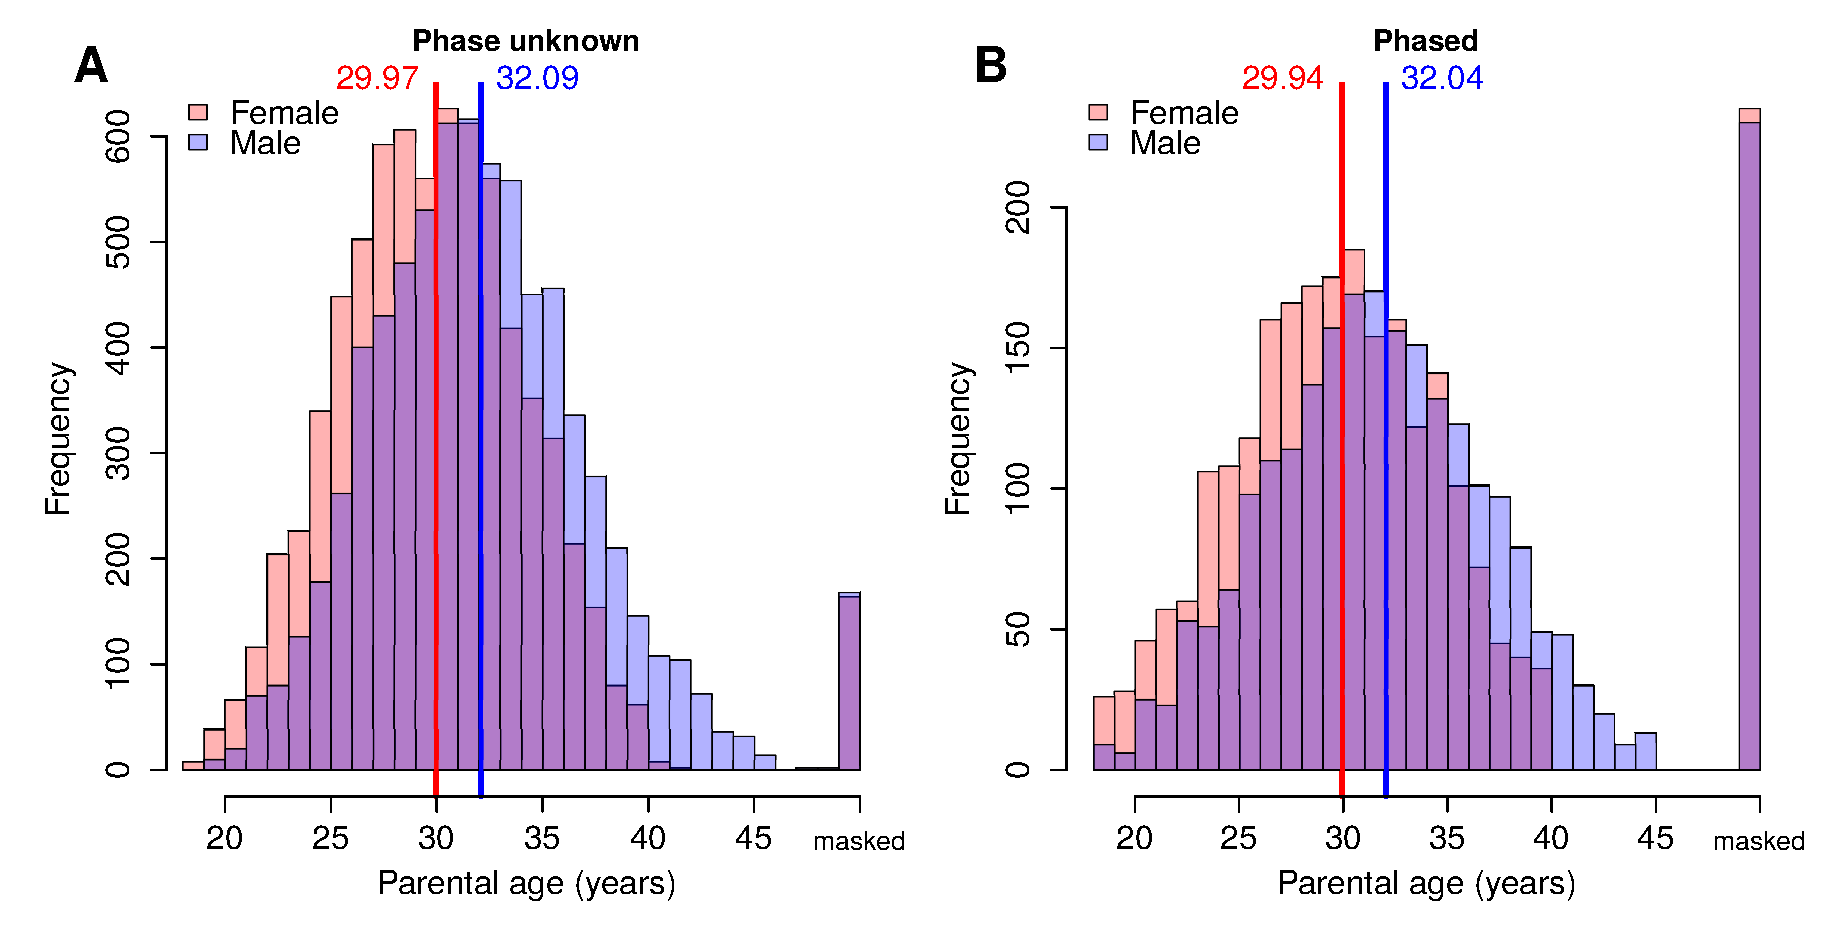
\includegraphics[width=\textwidth]{cointExtras/figs/ageHist_wMasked}
    \vspace{-20pt}
    \captionTitle{\textbf{Age distributions in the 23andMe dataset including older parents.}}{ 
        Phase-unknown parents are shown on the left panel (A), and phase-known parents, where ages were averaged across the children, are shown in the right panel (B).
        Additional data from older parents, in which the ages have been masked in females over 40 and males over 45 years old, are shown on the far-right of each distribution with the axis-label ``masked.''
        The vertical lines represent the mean of each distribution, excluding the older parents with masked ages.
    \label{fig:extrasAgeHist}}
\end{figure}
\clearpage}

\afterpage{
\begin{figure}[p]
    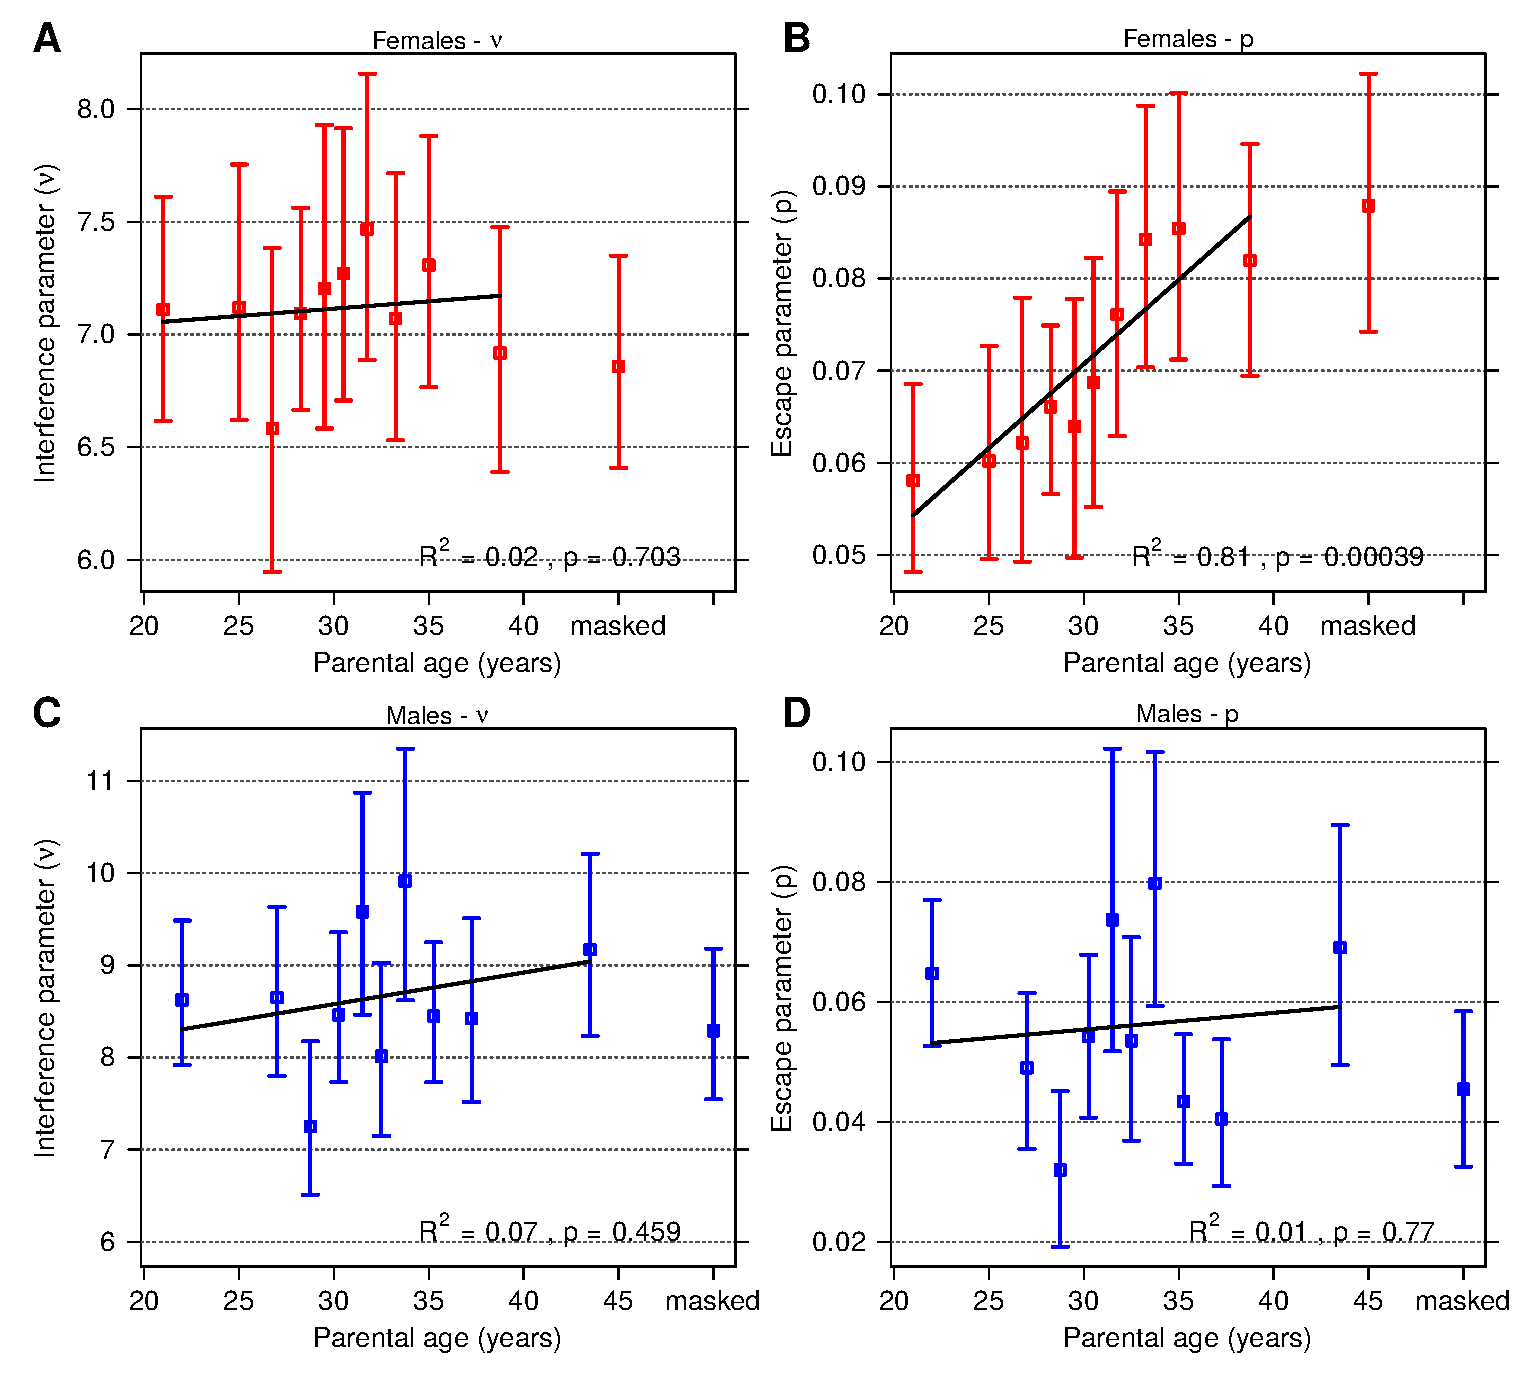
\includegraphics[width=\textwidth]{cointExtras/figs/coIntParam_wMasked}
    \vspace{-20pt}
    \captionTitle{\textbf{Crossover interference parameters as a function of age.}}{ 
        Parameter estimates for females are shown in the top two panels (A and B), males in the bottom two panels (C and D).
        Interference strength estimates ($\nu$) are shown in the left two panels (A and C), and estimates for the escape proportion are shown in the right panels (B and D).
        Data from older parents with masked ages are included in the plot with the axis label ``masked.''
        These older groups are excluded from the linear regression lines (shown in black).
    \label{fig:extrasCointAge}}
\end{figure}
\clearpage}



\afterpage{
\begin{figure}[p]
    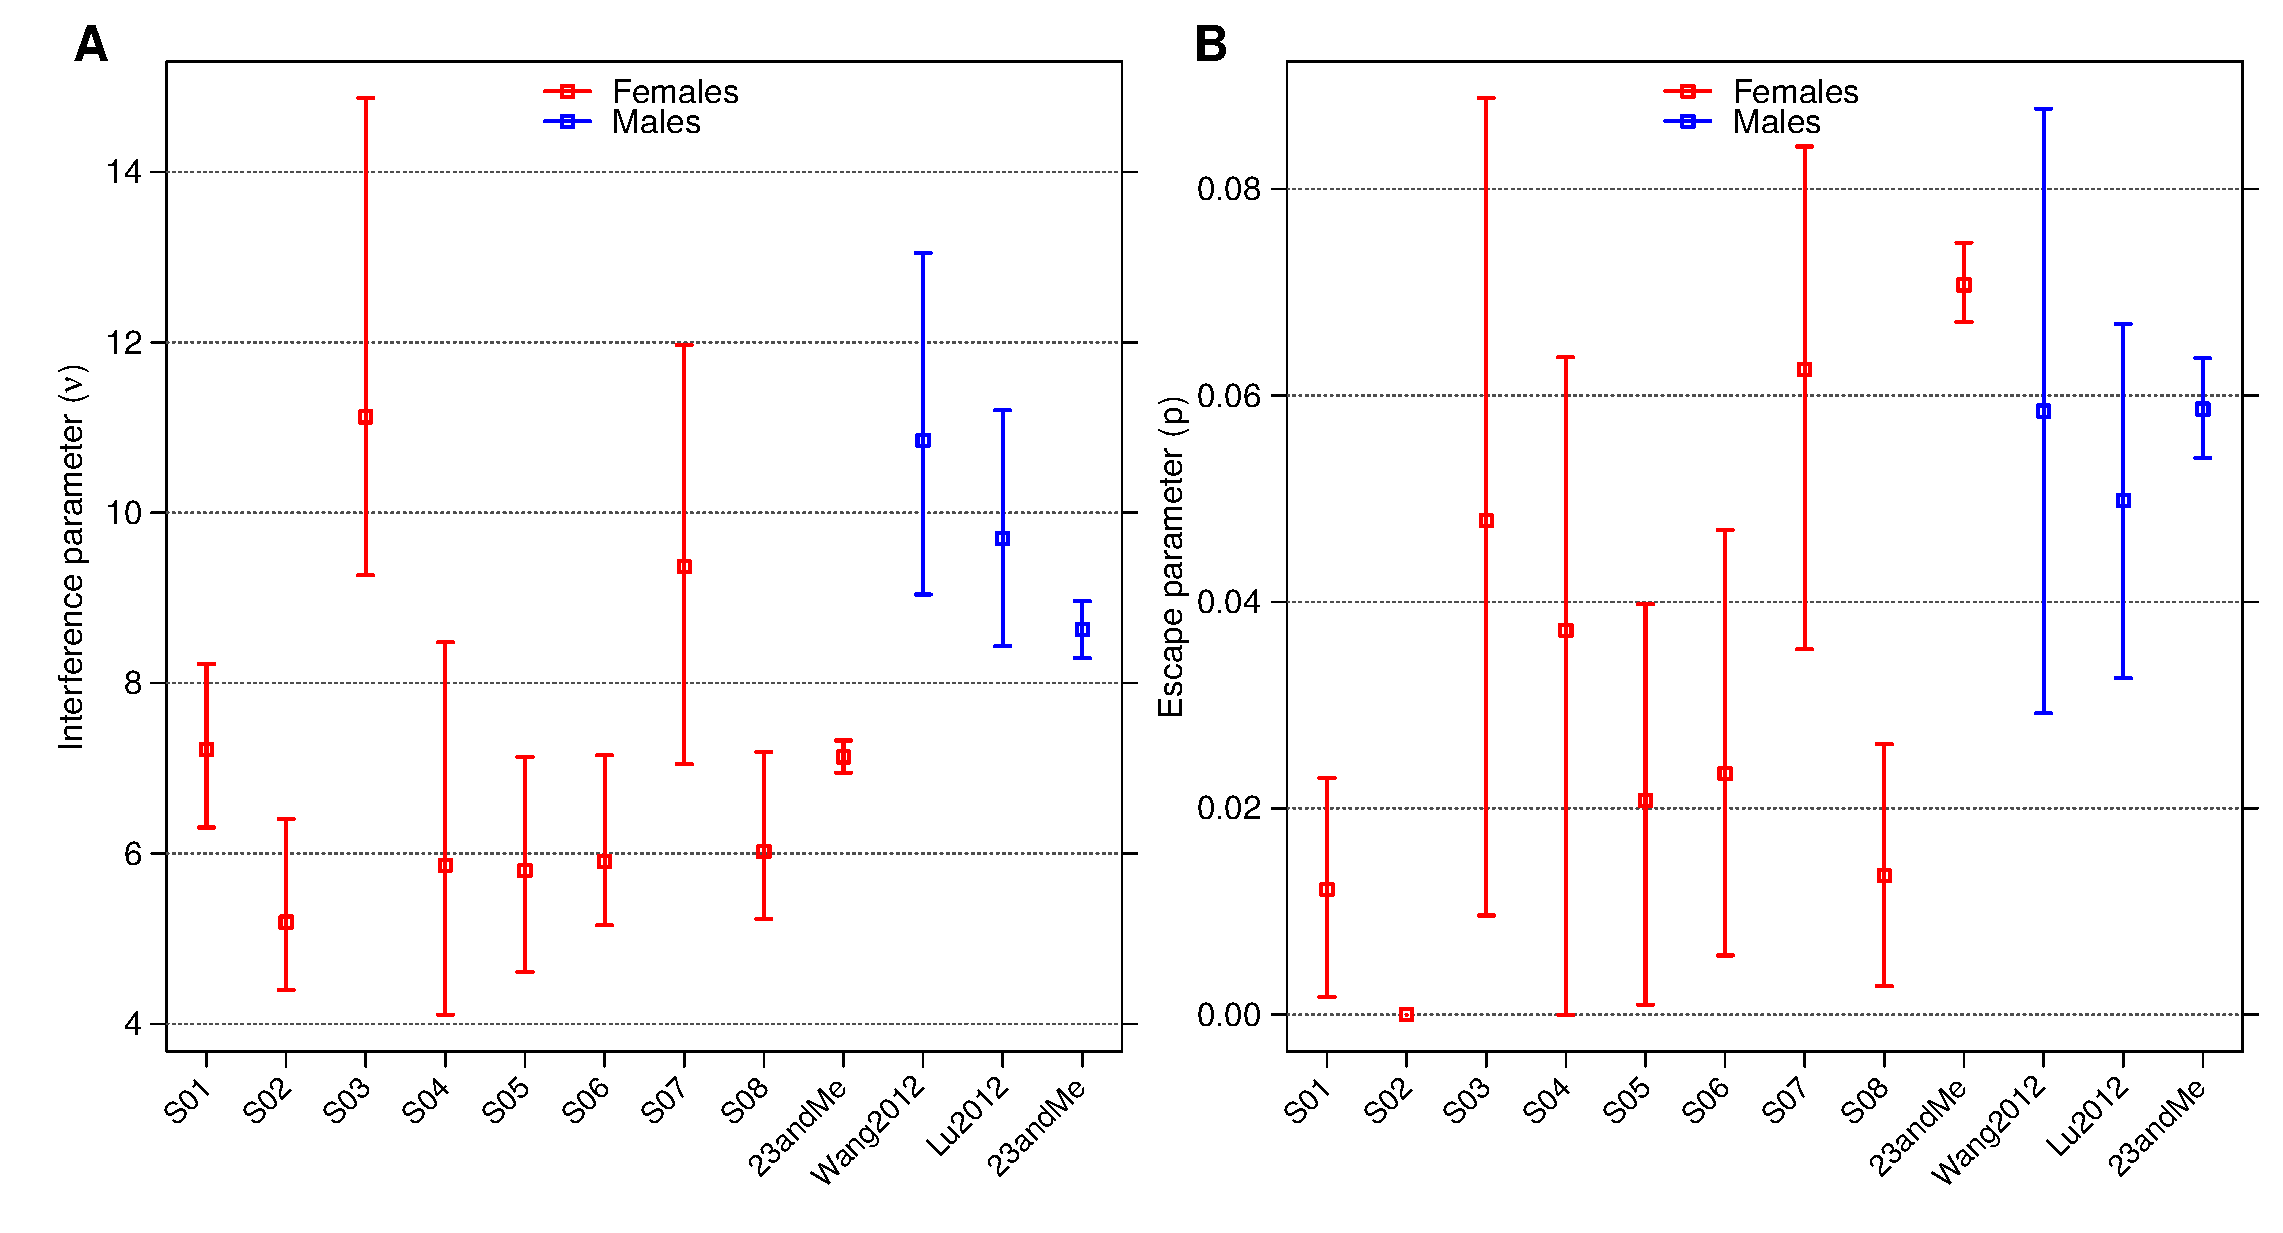
\includegraphics[width=\textwidth]{cointExtras/figs/coIntParam_public-individual}
    \vspace{-20pt}
    \captionTitle{\textbf{Crossover interference parameters in single cell data.}}{ 
        Interference parameter estimates are shown for the gamma escape model.
        The strength parameter is shown in panel A, and the escape parameter in panel B.
        Data points for females (red) represent data data generated by \citet{Hou2013}, representing 8 individuals.
        Data for males (in blue) comes from \citet{Lu2012} (n=99), \citet{Wang2012} (n=99).
        23andMe data\cite{Campbell2015} is provided for comparison and represents 2,184 females and 2,092 males).
    \label{fig:extrasCointSingle}}
\end{figure}
\clearpage}

% \subsection{Maternal age effect}

\clearpage
\section{Discussion}
The questions of how recombination properties vary on an individual basis and with age have long been outstanding.
I have presented here a series of analyses that attempt to shed light on these effects. %, some of which were addressed elsewhere in this thesis.

I have used an updated dataset which was previously presented without the age-masked individuals included here, both in this thesis (Chapter \ref{ch:cointEsc}), and in a peer-reviewed journal article\cite{Campbell2015}.
The original dataset was the first study of recombination in humans to find evidence for an increase in the proportion of events that escape crossover interference with increased age in females.
The original data was suggestive of an increasing de-regulation of events with age in females.
Considering the increased incidence of aneuploidy in older mothers\cite{Hassold2001}, it was suggested that these observations could be related.
Here, I have updated this finding to include data from older parents, which had been masked for privacy concerns.
The updated dataset validates and extends the original finding that interference escape increases in older mothers, but not fathers.
Although there is an overlap in the confidence intervals, the masked data in older mothers continues to increase from the previous bin and has no overlap with the youngest group, supporting the idea that the phenomenon is a linear increase.

In a separate analysis, I have taken previously published data from recombination studies that identified crossovers within individuals using multiple single cell assays.
These data provide a picture of how much variation can be expected within a single individual, which appears to vary substantially.
Although the number of individuals represented here is small, the techniques used to produce this data provide a promising avenue for future research as the cost and complexity to perform these analyses decreases.
In the future, such analyses could be performed on a much larger scale, and provide valuable insight into the variation of recombination properties within individuals.

\clearpage
\renewcommand{\bibname}{References}
\bibliographystyle{ccampbell_thesis}
\begingroup
    \setlength{\bibsep}{10pt}
    \linespread{1}\selectfont
    \bibliography{/home/ccampbell/Dropbox/papers/thesis-cointExtras}
\endgroup



